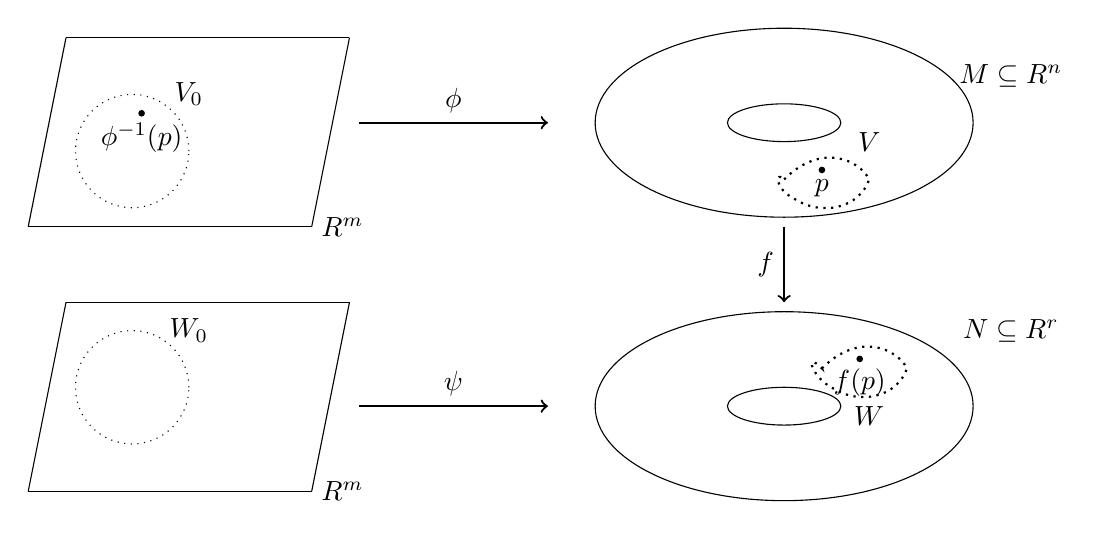
\begin{tikzpicture}[scale=1.2]

% --- Dominio en R^2 ---
\begin{scope}
  \draw[-] (0,0.4) -- (3,0.4) node[right] {$\mathbb{R}^{m}$};
  \draw[-] (0.4,2.4) -- (3.4,2.4);
  \draw[-] (3,0.4) -- (3.4,2.4);
  \draw[-] (0,0.4) -- (0.4,2.4);

  % Abierto (rectángulo)
  \draw[dotted] (1.1,1.2) circle (0.6);

  \node at (1.7,1.8) {$V_0$};
\end{scope}

% Flecha phi
\draw[->, thick] (3.5,1.5) -- (5.5,1.5) node[midway, above] {$\phi$};

% --- Toro (aproximación 2D) ---
\begin{scope}[xshift=8cm]

  % Contorno exterior (elipse grande)
  \draw (0,1.5) ellipse (2 and 1);

  % Agujero interior
  \draw (0,1.5) ellipse (0.6 and 0.2);

\draw[dotted, thick]
  (0,0.9)
  .. controls (0.4,1.3) and (0.8,1.1) ..
  (0.9,0.9)
  .. controls (0.8,0.6) and (0.4,0.5) ..
  (0.1,0.7)
  .. controls (-0.1,0.8) and (-0.1,1) ..
  cycle;

\node at (0.9,1.3) {$V$};
\node at (2.4,2) {$M\subseteq \mathbb{R}^{n}$};
\end{scope}

% Segunda

\begin{scope}
  \draw[-] (0,-2.4) -- (3,-2.4) node[right] {$\mathbb{R}^{m}$};
  \draw[-] (0.4,-0.4) -- (3.4,-0.4);
  \draw[-] (3,-2.4) -- (3.4,-0.4);
  \draw[-] (0,-2.4) -- (0.4,-0.4);

  % Abierto (rectángulo)
  \draw[dotted] (1.1,-1.3) circle (0.6);

  \node at (1.7,-0.7) {$W_0$};
\end{scope}

% Flecha phi
\draw[->, thick] (3.5,-1.5) -- (5.5,-1.5) node[midway, above] {$\psi$};

% --- Toro (aproximación 2D) ---
\begin{scope}[xshift=8cm]

  % Contorno exterior (elipse grande)
  \draw (0,-1.5) ellipse (2 and 1);

  % Agujero interior
  \draw (0,-1.5) ellipse (0.6 and 0.2);

\draw[dotted, thick]
  (0.4,-1.1)
  .. controls (0.8,-0.7) and (1.2,-0.9) ..
  (1.3,-1.1)
  .. controls (1.2,-1.4) and (0.8,-1.5) ..
  (0.5,-1.3)
  .. controls (0.3,-1.2) and (0.2,-0.9) ..
  cycle;

\node at (0.9,-1.6) {$W$};
\node at (2.4,-0.7) {$N\subseteq \mathbb{R}^{r}$};
\end{scope}

\draw[->, thick] (8,0.4) -- (8,-0.4) node[midway, left] {$f$};

\fill (1.2,1.6) circle (1pt);
  \node[below] at (1.2,1.6) {$\phi^{-1}(p)$}; 

\fill (8.4,1) circle (1pt);
  \node[below] at (8.4,1) {$p$}; 

\fill (8.8,-1) circle (1pt);
  \node[below] at (8.8,-1) {$f(p)$}; 
\end{tikzpicture}
